\documentclass[pdftex,12pt,a4paper]{article}
\usepackage{url}
\usepackage{natbib}
\usepackage[pdftex]{graphicx}
\usepackage{float}
\renewcommand*{\bibfont}{\raggedright}
\newcommand{\HRule}{\rule{\linewidth}{0.5mm}}

\author{
  Pratyaksh Sharma\\
  120050019\\
  pratyaksh@cse.iitb.ac.in
  \and
  Sanket Kanjanlkar\\
  120050011\\
  sanket@cse.iitb.ac.in
  \and 
  Shirish Namdeo\\
  110050040\\
  shirishkumar@cse.iitb.ac.in
}
\title{\HRule \\[0.4cm]{ \huge \bfseries Steam locomotive simulation in Box2D \\[0.4cm] }\HRule \\[1.5cm]}
\date{9 April, 2014}


\begin{document}
\maketitle
\begin{abstract}
\indent \par{A steam locomotive is quite a complex machine and comes in a variety of designs. Various designs either differ in the driving wheel and driving rod mechanism (motion of wheels controlled by locomotive's pistons) or in the steam engine itself (which usually consists of a piston-cylinder arrangement coupled with valve rods). Box2D is a popular 2D physics simulator engine, a simulator of choice for games building upon physics. Here we have simulated a simple model of a steam locomotive in Box2D.}
\end{abstract}

\tableofcontents

\pagebreak

\section{Introduction}
\par{A steam locomotive is a powered railway vehicle used for pulling trains. It uses an engine that uses the expansion or rapid condensation of steam to generate power. The classical steam engine consists of an iron cylinder, piston, connecting rod and beam or a crank and flywheel, and miscellaneous linkages. Steam is alternately supplied and exhausted by one or more valves.}
\par{The engine requires a heat source which is usually burning coal and a boiler which uses this heat to boil water to produce steam. This steam is directed into a chamber of one or more pistons and valves. Also, a cold sink is onboard which condenses the produced steam after it is exhausted.}
\par{For the current simulation we have omitted burning coal, the boiler and the cold sink part.}

\section{Original design proposal}
\par{Figure 1 shows the design of the locomotive as proposed earlier\cite{youtube1}. At first we tried to simulate exactly this model in Box2D, but things were not that simple.}

\subsection{Interesting observations}
\par{Both the driving rod-wheel mechanism and the steam engine are oversimplifications of a real steam locomotive and they lack many components essential in proper functioning of the machine.}
\subsubsection{Driving rod mechanism}
\par{The driving rod mechanism consists of two parts: rods connected to the piston rod and those connected to valve rod.}
\par{Piston rod pushes rod2 which in turn pushes rod 1. Now rod1 is connected to all three wheels and its motion is constrained in such a manner that the wheels turn and the locomotive moves forward. This basic design of the piston rod part just works fine.}

\par{The motion of rod1 should affect that of rod3 and rod4 in a manner such that valve rod is pushed to the right. We realize that only rod3 and rod4 are not sufficient to maintain the phase difference between piston and valve rods. A more complex system of rods is needed for the valve part to work.}

\begin{figure}[H]
\centering
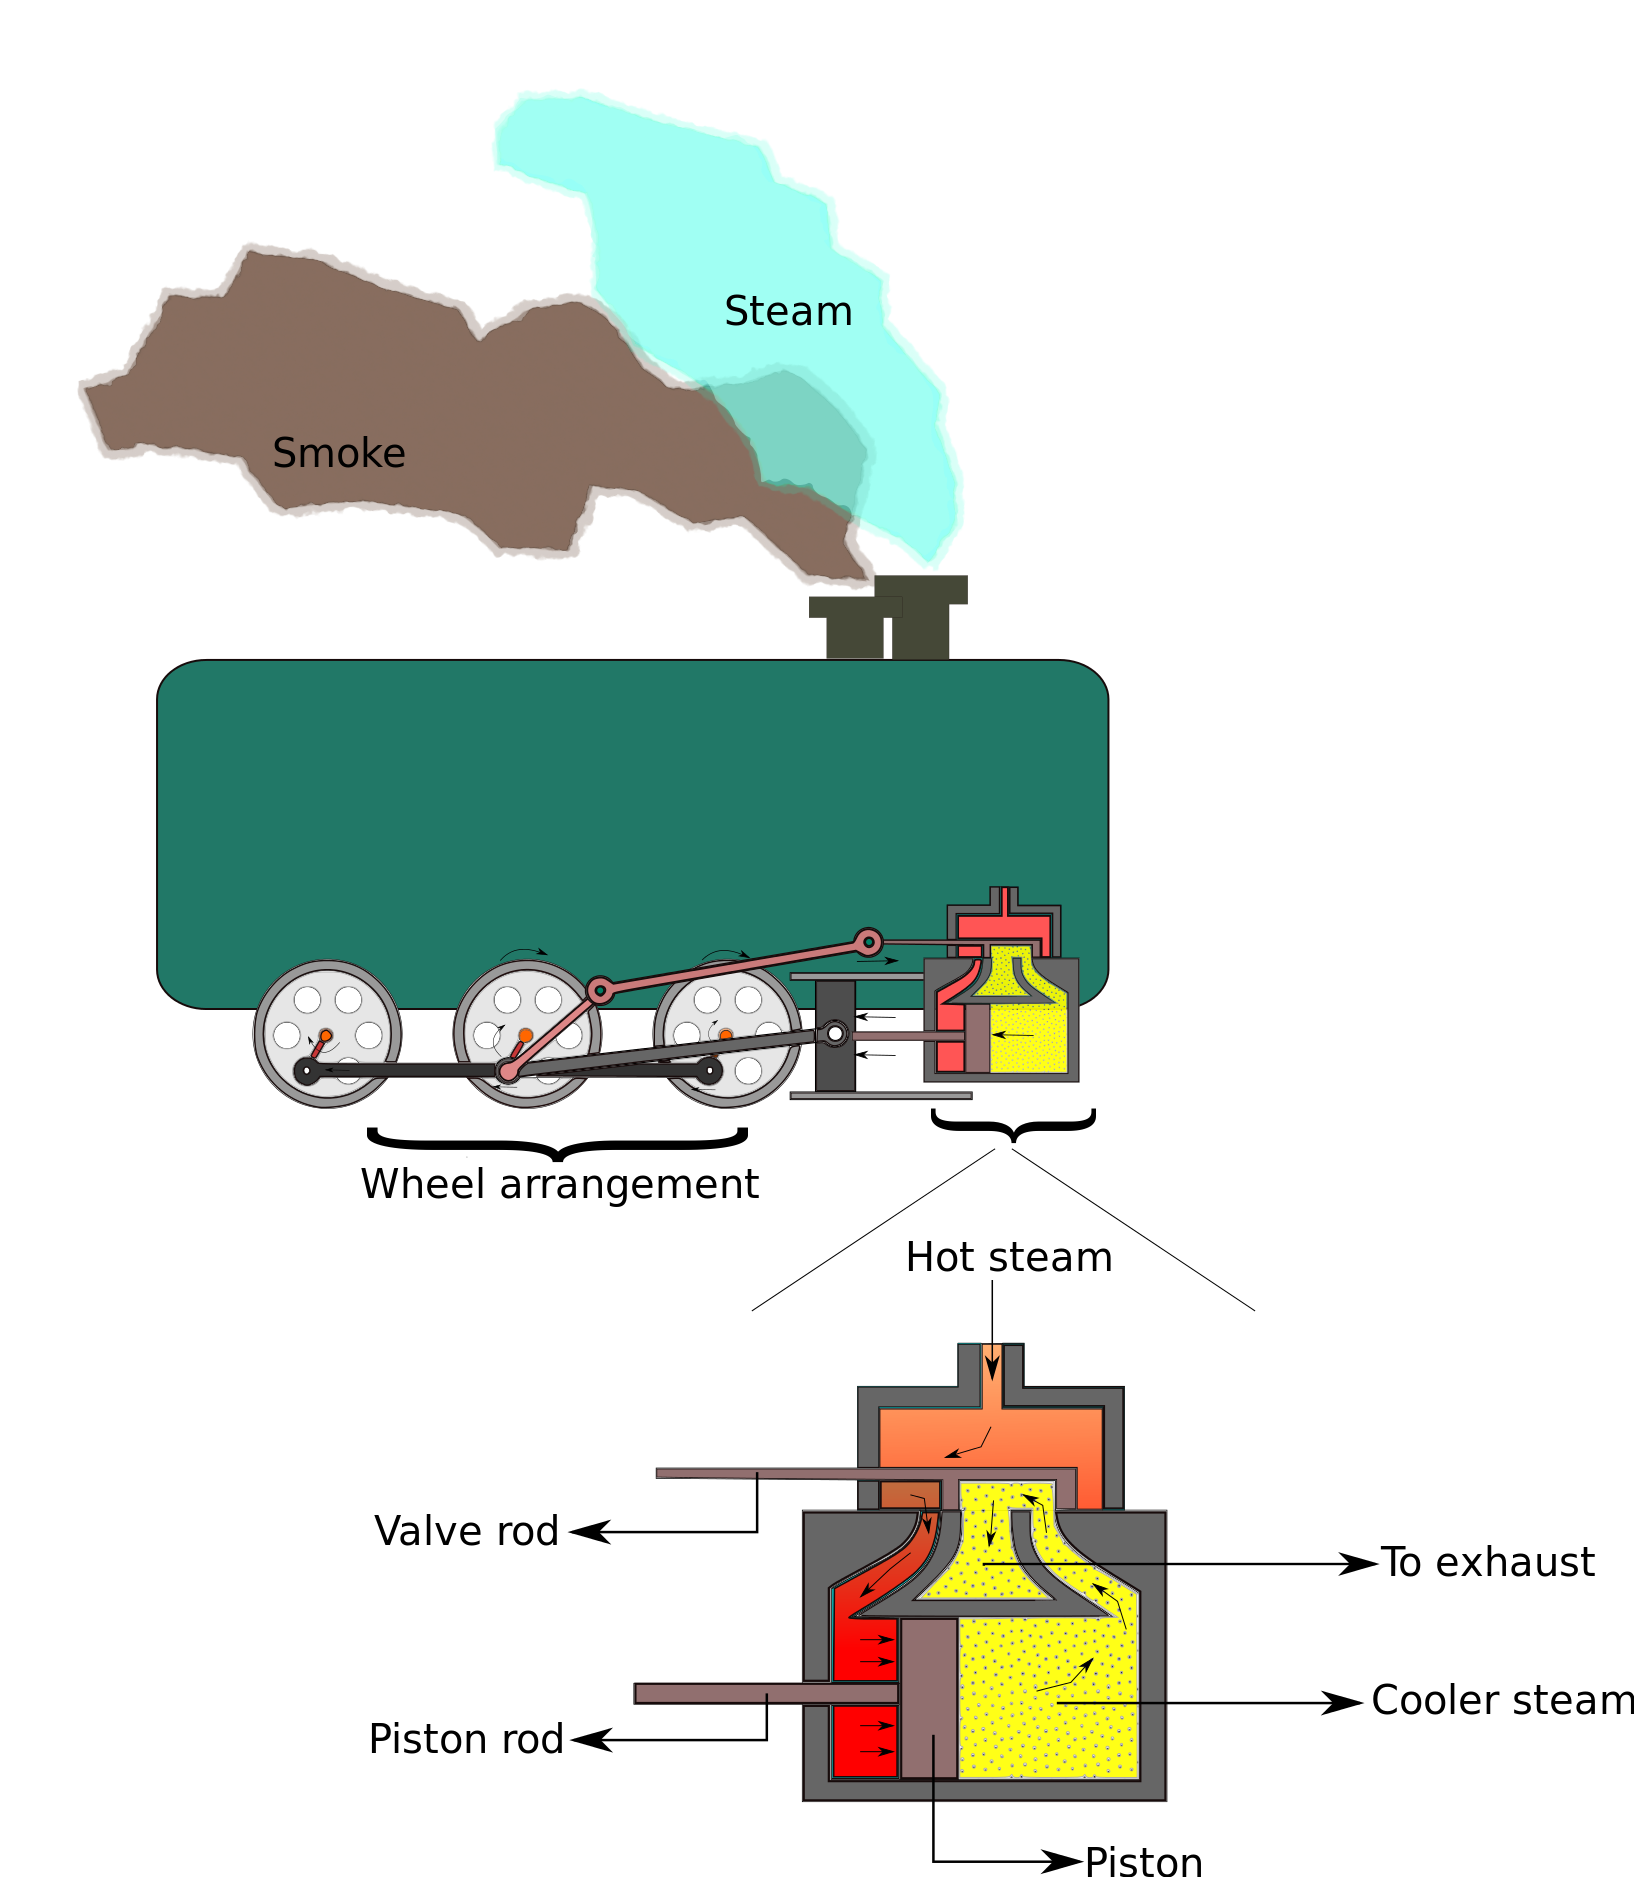
\includegraphics[scale=.23]{../images/steameng.png}
\caption{Original Design}
\end{figure}

\subsubsection{Engine}
\par{As can be seen in Figure 1, the position of exhaust is somewhat arbitrary. Also, one can't see how the exhaust connect to the chimney on the roof of the locomotive. This design requires that valve rod and piston rod be completely out of phase (when valve rod moves left, piston rod moves right and vice versa).}

\begin{figure}[H]
\centering
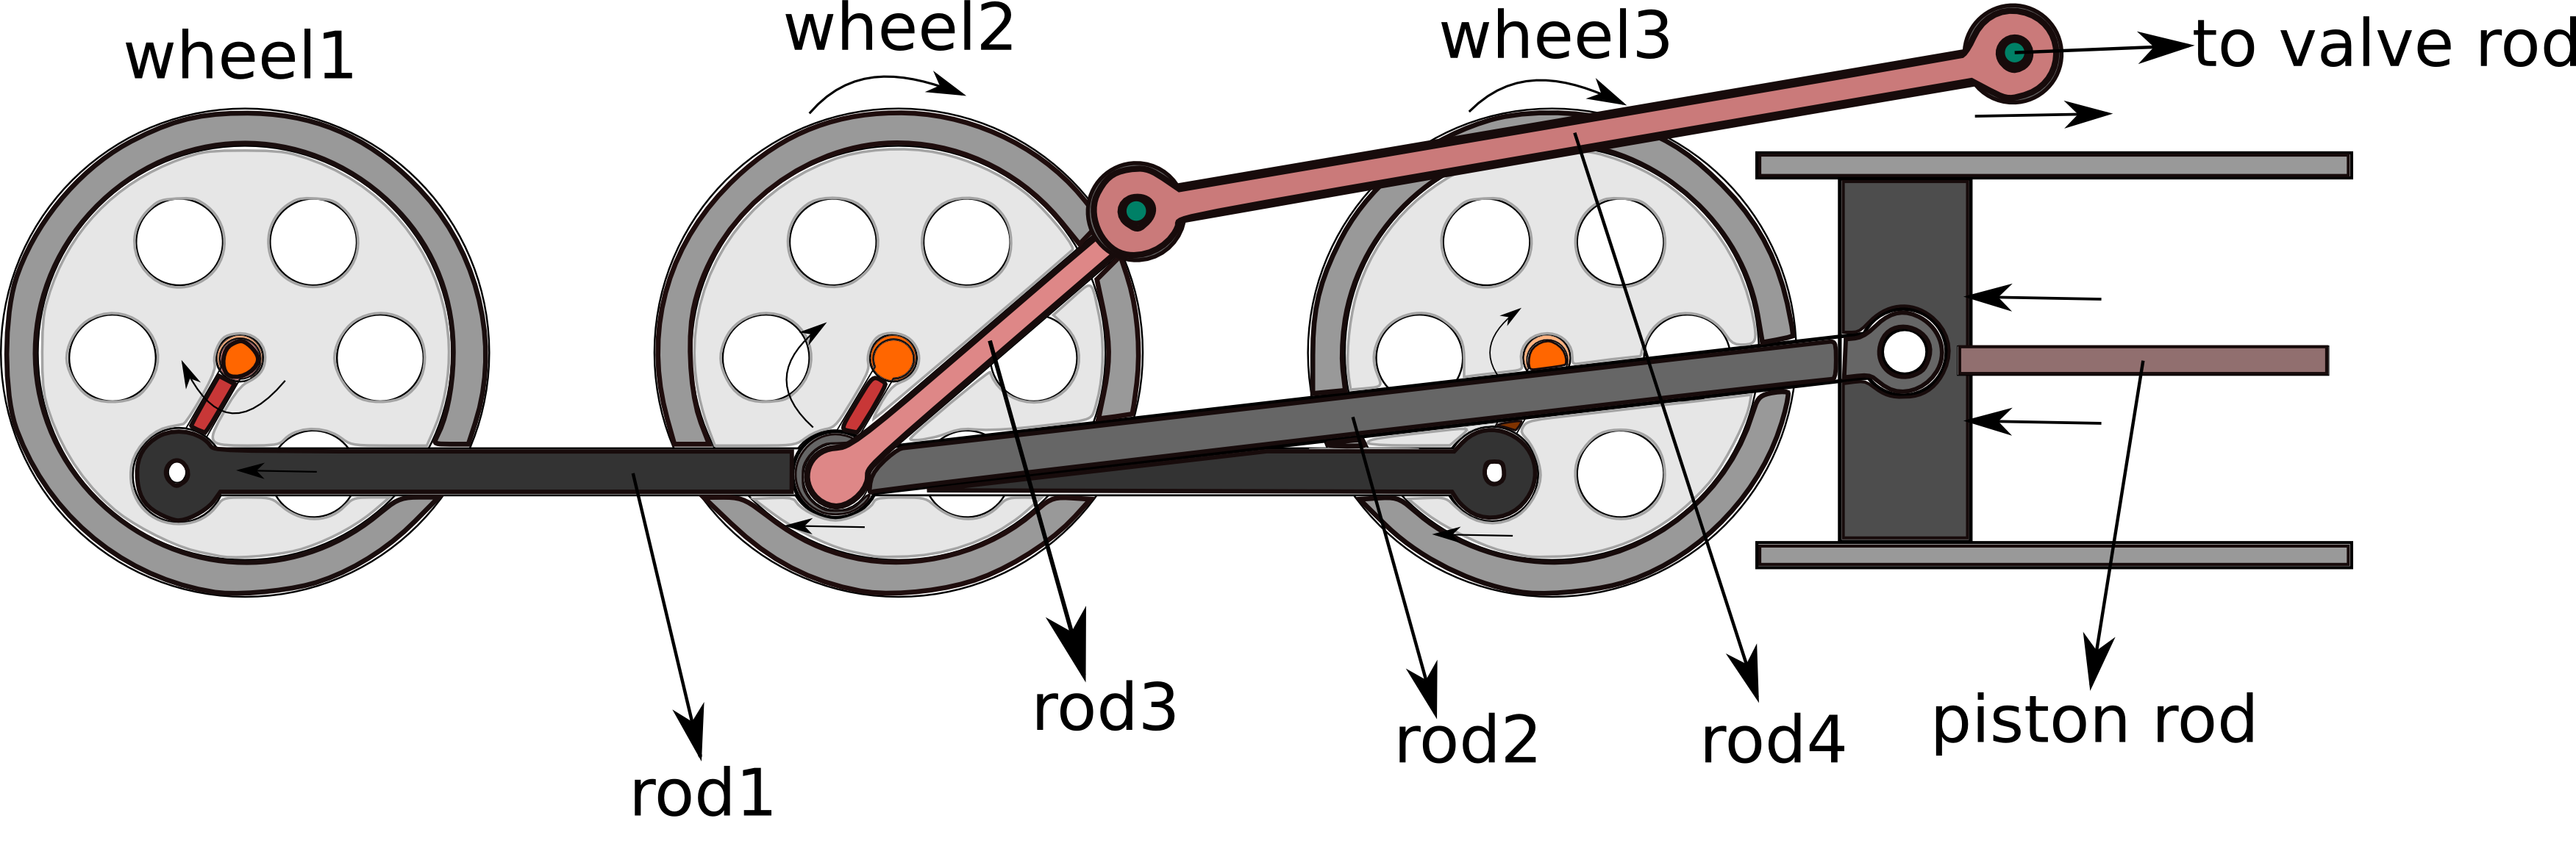
\includegraphics[scale=.60]{../images/oldlabel.png}
\caption{Wheel mechanism}
\end{figure}

\section{The design implemented}

\par{Figure 3 shows the final design.\cite{model1}}

\begin{figure}[H]
\centering
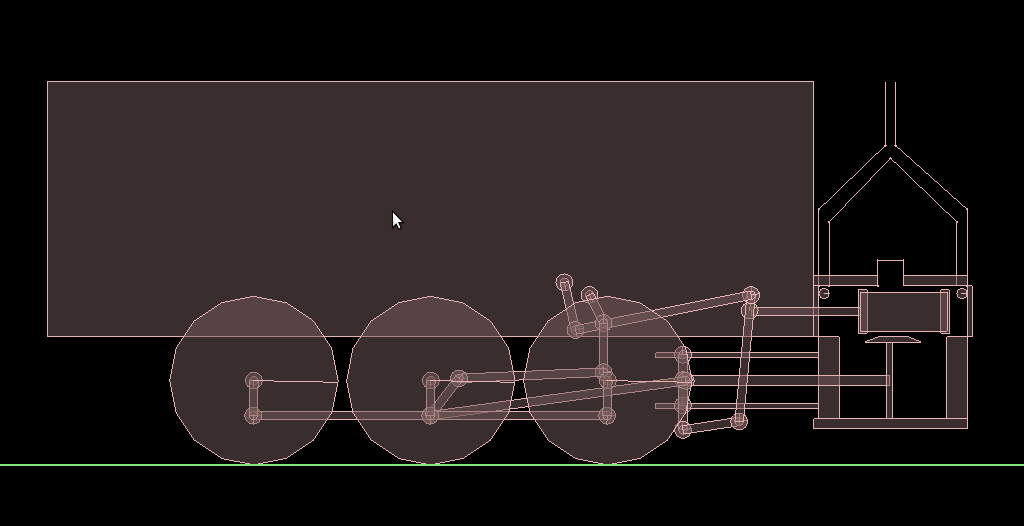
\includegraphics[scale=.37]{../images/slnew.png}
\caption{Showing initial position of locomotive}
\end{figure}

\subsection{Observations}
\par{The design of both the engine part and the driving rod mechanism were modified such that the valve and exhaust systems function properly.}

\subsubsection{Driving rod mechanism}

\par{As can be seen, several rods are employed to control the motion of the valve. In total the combined motion of 8 rods controls the valve. Most of these have joints at the ends about which the connected bodies are free to rotate. Rest of the rods have one joint which welds them to the locomotive or to one of the wheels.}

\begin{figure}[H]
\centering
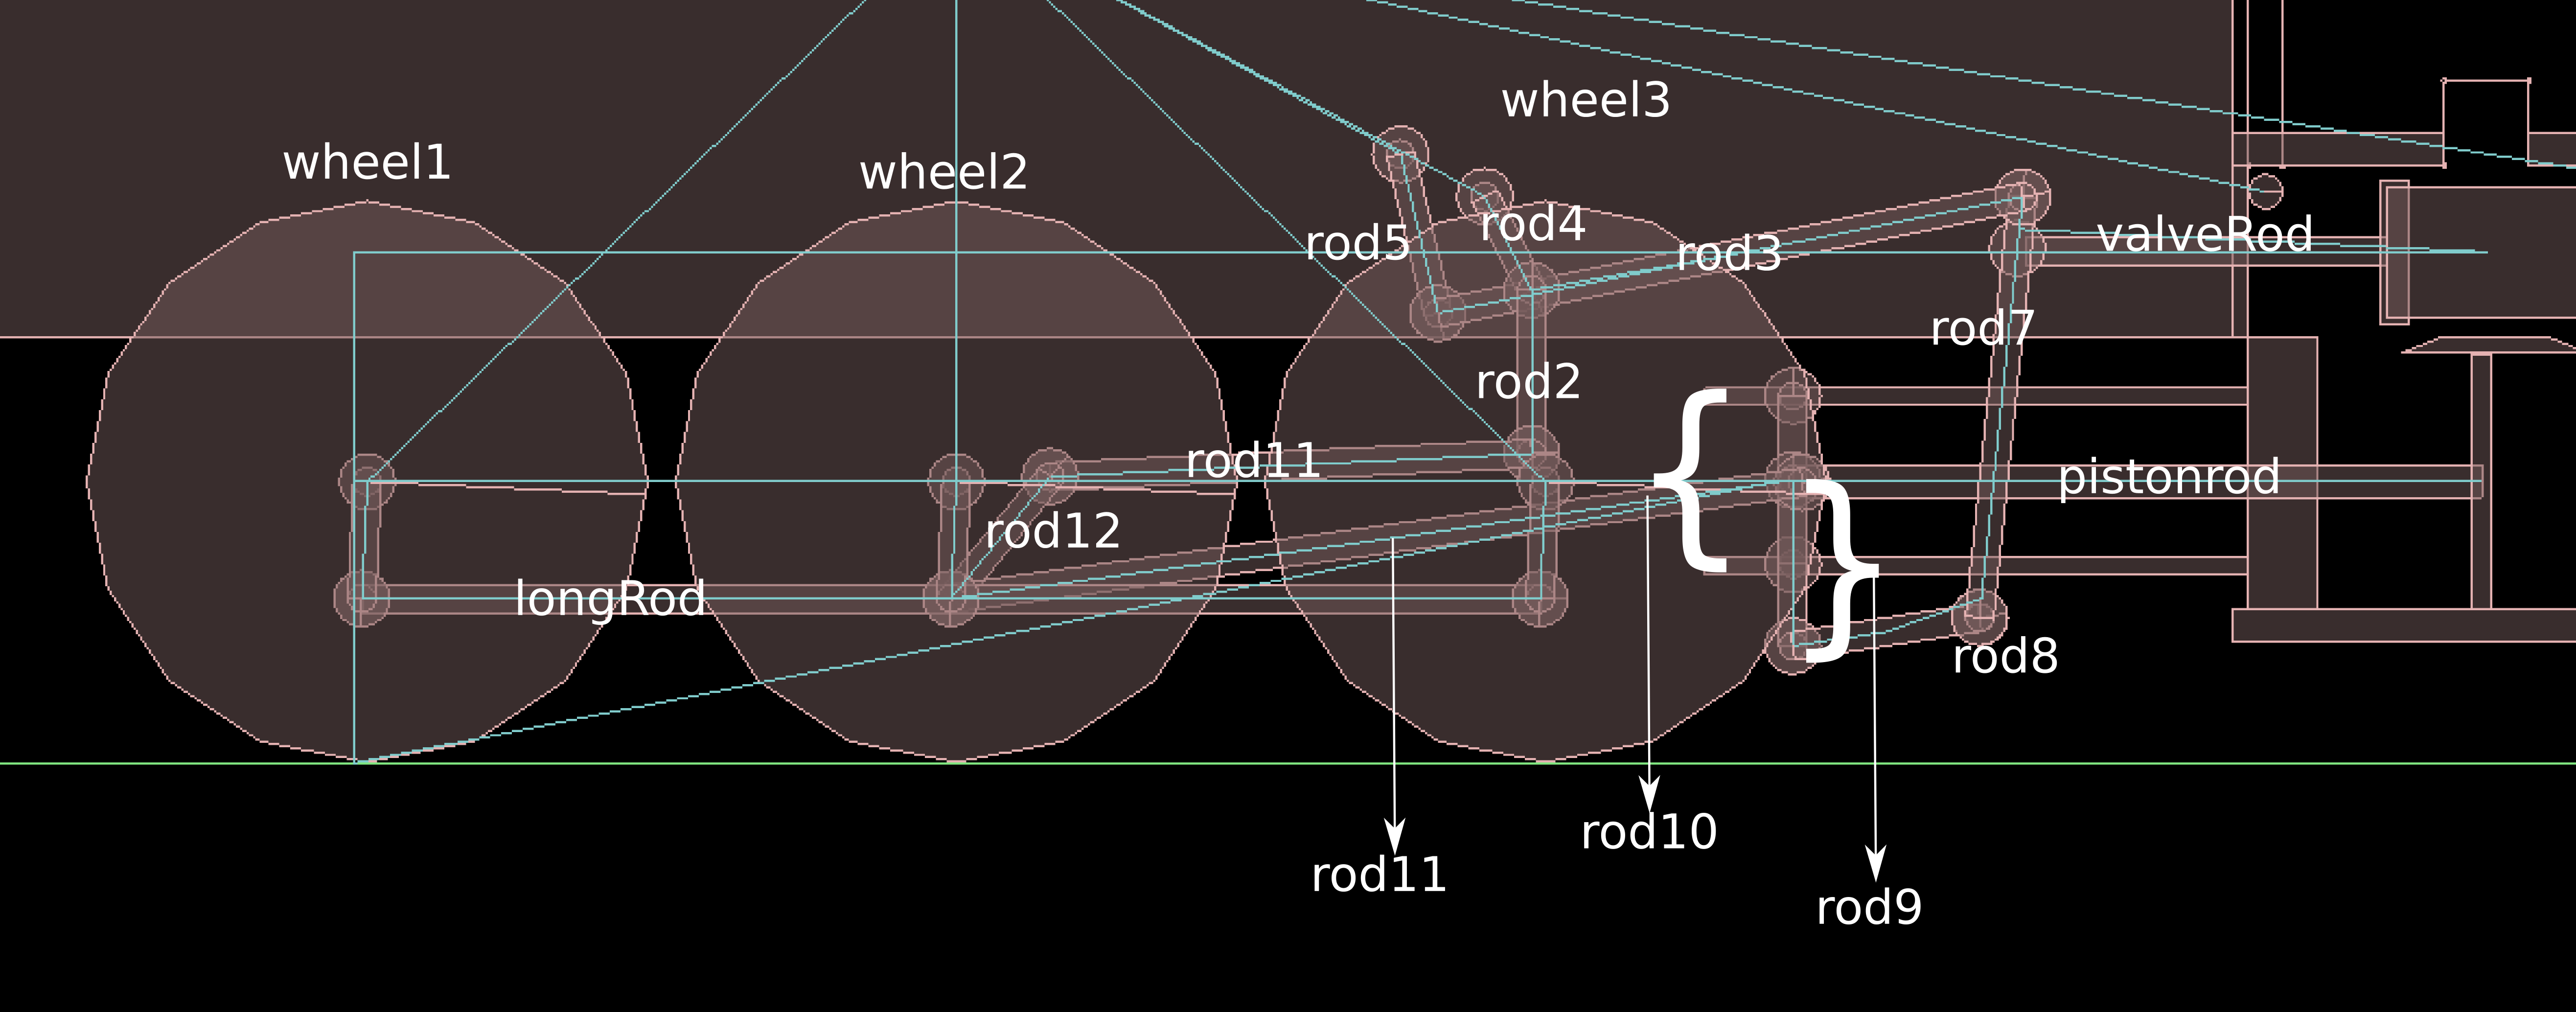
\includegraphics[scale=.37]{../images/labels.png}
\caption{Rod names, same as those used in code}
\end{figure}

\par{The valve rod is connected near the top end of rod7 with a revolute joint. The motion of rod7 governs the motion of the valve rod. The motion of rod7 is in turn governed by the motion of rod3 and rod8 which are connected at the end points of rod7 with revolute joints.}
\par{rod10 is a vertical rod which slides on two rails (parallel to the ground) that are fixed to the locomotives body. To ensure horizontal motion of rod10, a prismatic joint is created between the ground and rod10. The center of rod10 welds at its center rod9 and the piston rod. rod11 is also connected to the center of rod10 but by a revolute joint. In this way, the piston rod drives rods 10, 9 and 11. But rod11 is connected to the longRod, so the motion of the piston rod indirectly turns the wheels.}
\par{The top ends of rod5 and rod4 are welded to the locomotive body. The bottom end of rod4 and top end of rod2 are also welded.}
\par{Both ends of rod12 are welded to the middle wheel. rod1 connects bottom end of rod2 with top end of rod12 both with revolute joints.}
\par{The lengths and positions of all the rods ensure that the piston rod and valve rod remain in phase for the duration of a cycle, and that the motion of piston rod turns the wheels in the clockwise direction.}

\subsubsection{Engine}
\par{The engine design\cite{youtube2} has changed considerably from the previous one. Refer Figure 5.}
\begin{figure}[H]
\centering
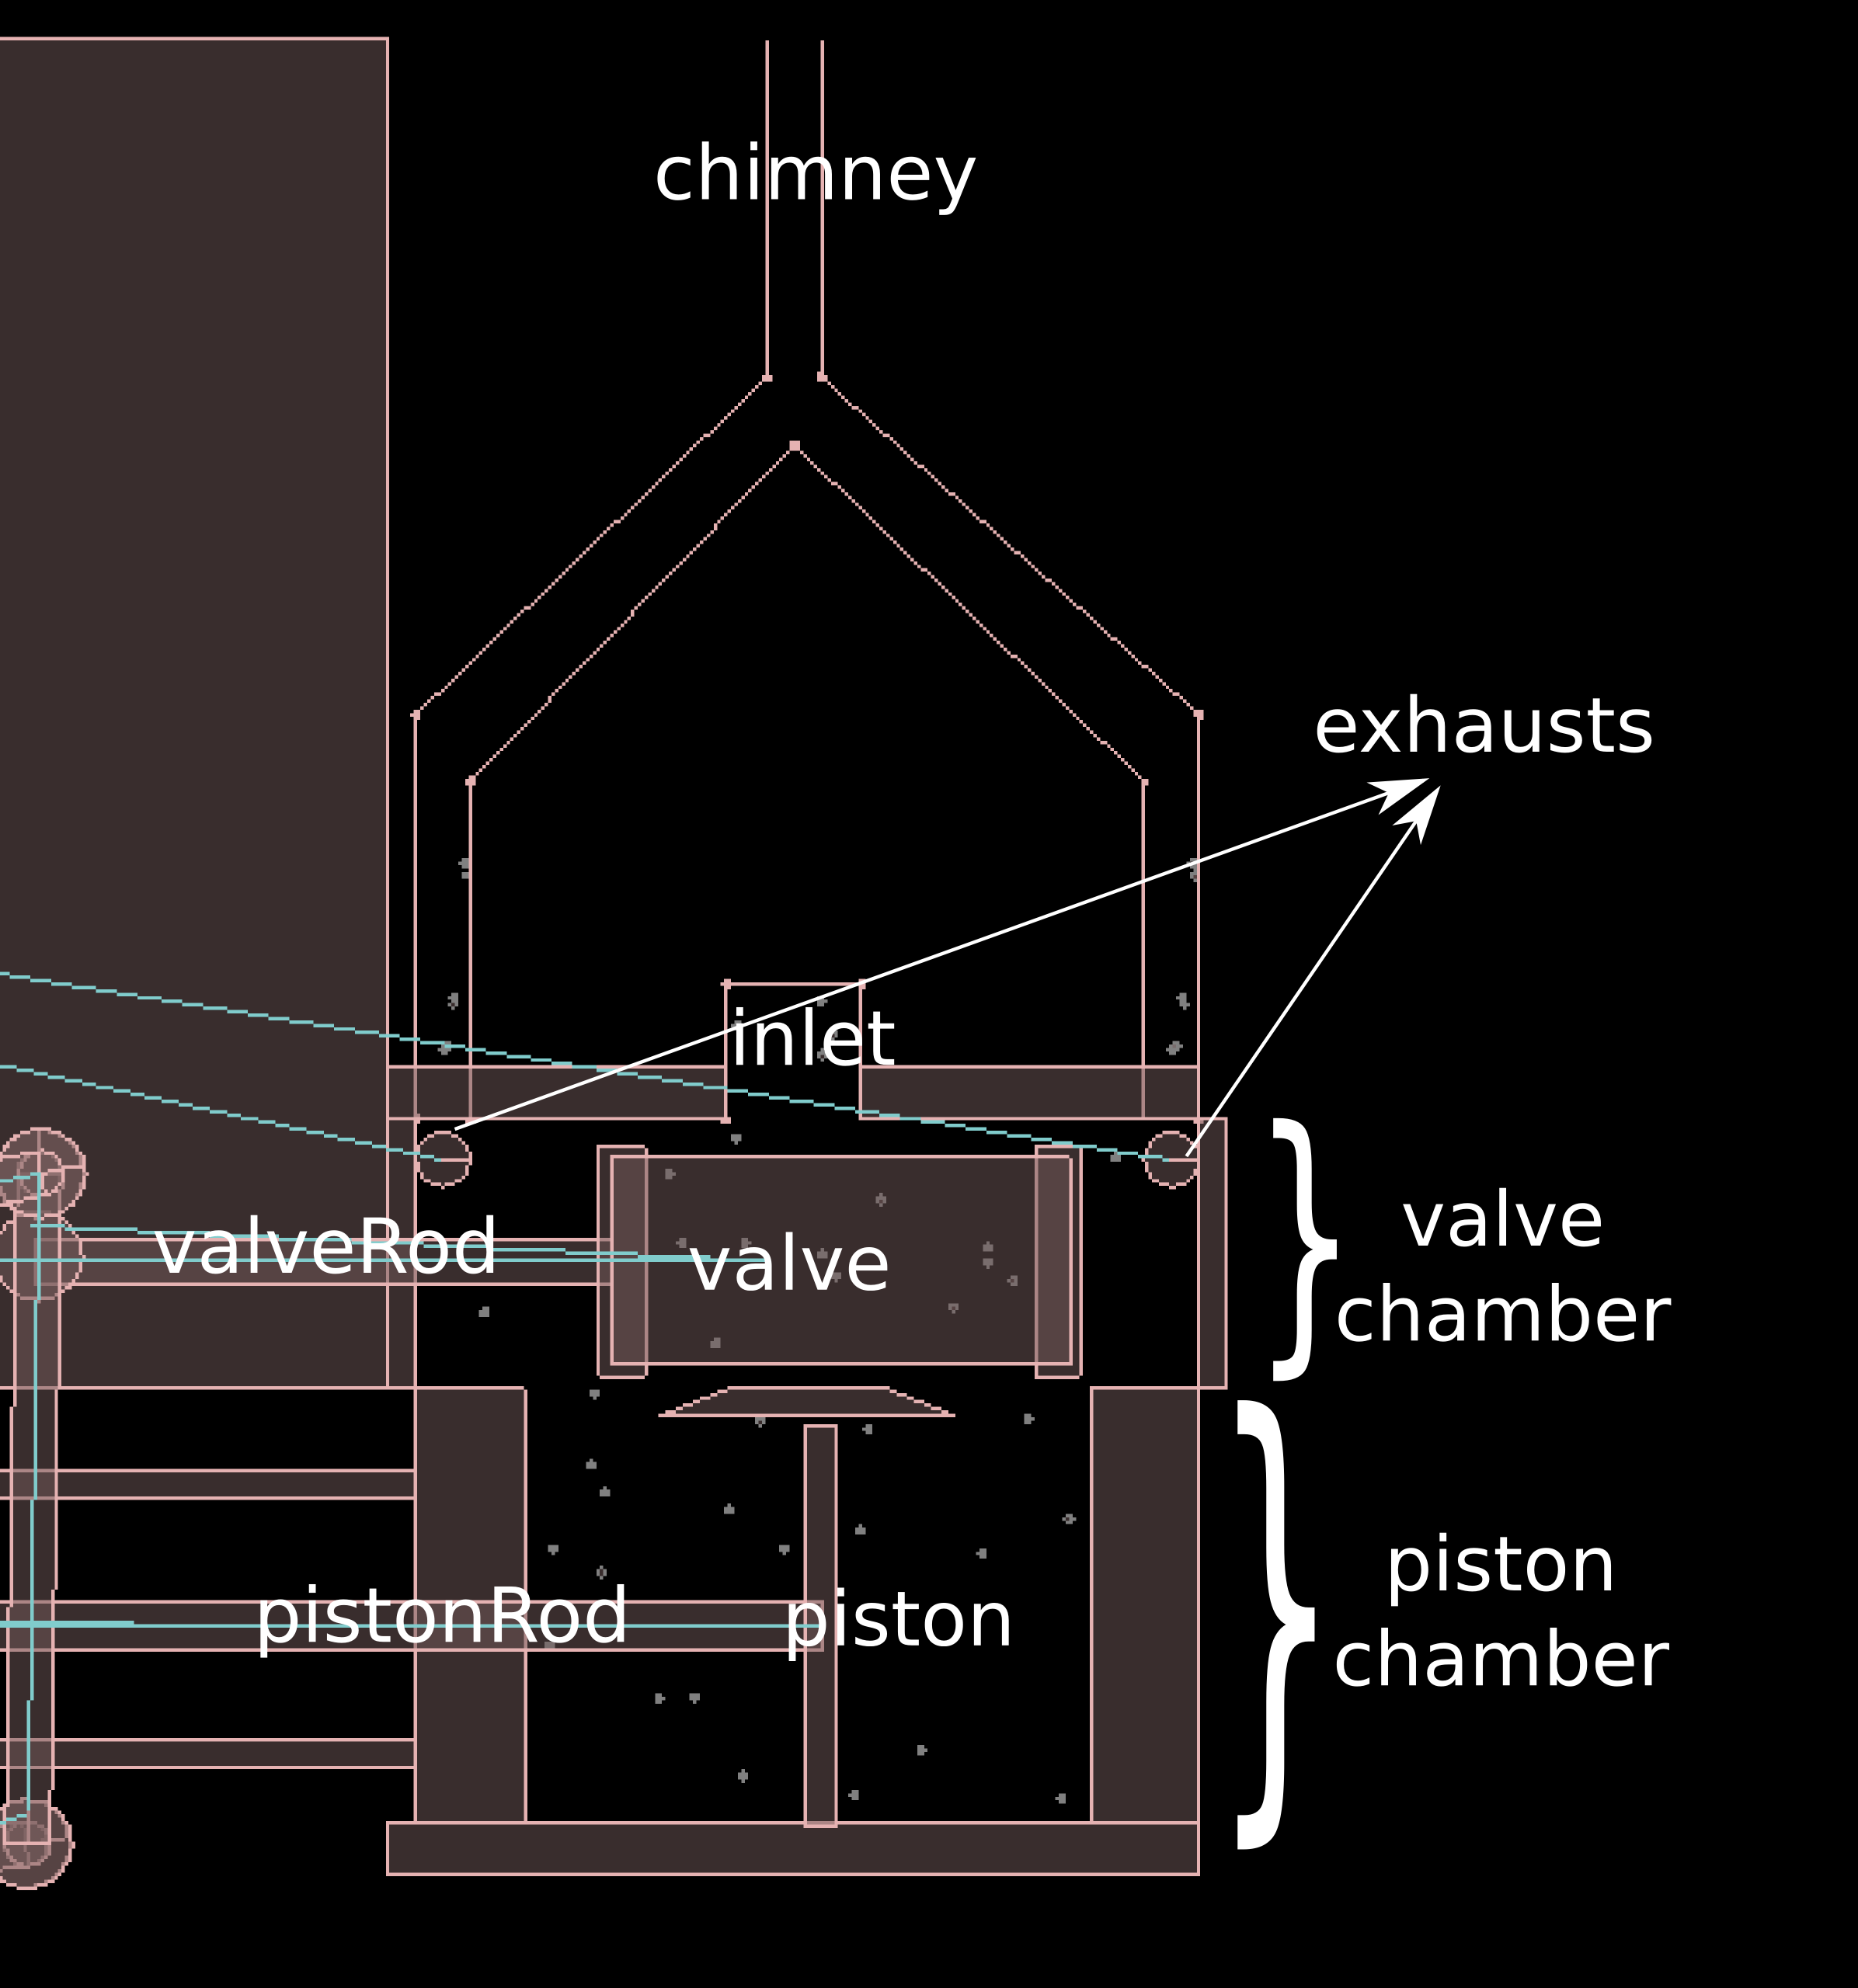
\includegraphics[scale=.37]{../images/enginelabels.png}
\caption{Engine labels}
\end{figure}
\par{Two exhaust are placed at the top ends of the valve cylinder. The particles to be exhausted are directed from these to a chimney located above the valve cylinder.}
\par{Particles are created at the inlet and are intialized with random direction and fixed speed. The particles travel through the engine interior. Particles collide with engine walls and impart momemtum to piston rod. Finally when the particles collide with the exhaust system, they get deleted. For every particle deleted, a new particle is created near the corresponding exhaust pipe and get released as smoke.}

\section{About the code}
\par{All bodies in the simulation are dynamic. The driving rod mechanism consists of several rods. All the rods have same shape, they differ only in their dimensions, positions and joints. The creation of these rods is facilated by C++ macros, which help make the code brief and neat.}

\par{Particles are modelled as circles with small radius. Also the particles are set with user data 1 and are set as bullets.	Entire engine is implemted as one body with multiple fixtures. A custom contactListner class\cite{contactlistener} has been implemeted . The  begincontact function has been overridden so that it counts the number of particles that collide with a particular exhust. This function also pushes the particles to be deleted to a vector del\_list. The particles in the del\_list are then deleted in the Step()function. A custom data structure has been implemented to save the time of creation of bodies created near exhuast a. The smoke data structure has two fields b2Body* body and time\_stamp. Particles are then deleted from this queue after 200 steps. time\_step\_count maintains the number of times step function is called. The color of particles has also been changed to grey by changing the definition of DrawSolidCircle in render.cpp.}

\section{Timing}
\par{For the following analysis, we have used no. of iterations = 500 and no. of reruns = 10.}
\subsection{Analysis of Loop time vs No. of iterations}

\begin{figure}[h!]
\centering
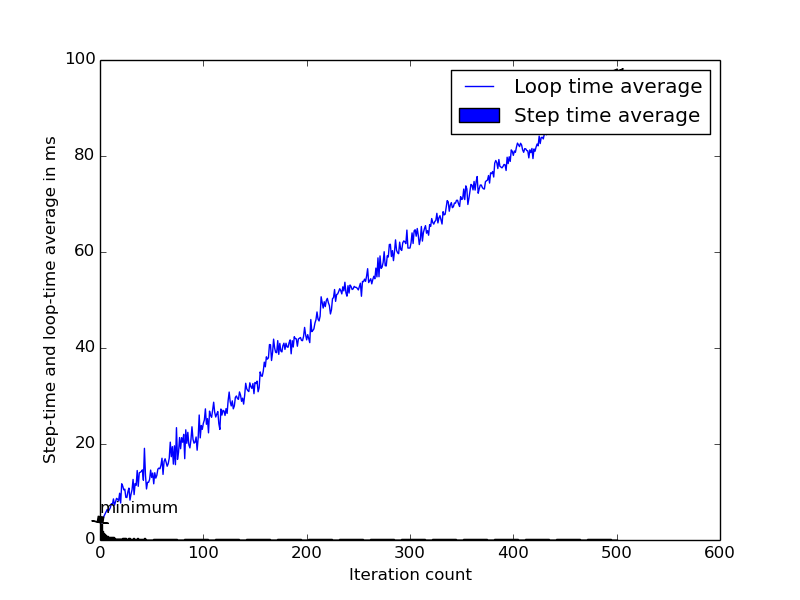
\includegraphics[scale=.60]{../images/plot01.png}
\caption{plot01}
\end{figure}

\par{The average step time almost remains constant. We obtain more accurate data as we take further iterations into account.} 

\par{The total loop time increases almost linearly. There are some ups and downs in the line graph which indicates that the solver is only invoked when it is needed. In some particular iteration, where more collisions occur (and/or more objects move) take longer time for solver to solve and hence there is some variation in the (almost) linear loop time.}

\subsection{Observations from graph of Step time, Collision time, Velocity time, Position time vs Iteration values}
\begin{figure}[h!]
\centering
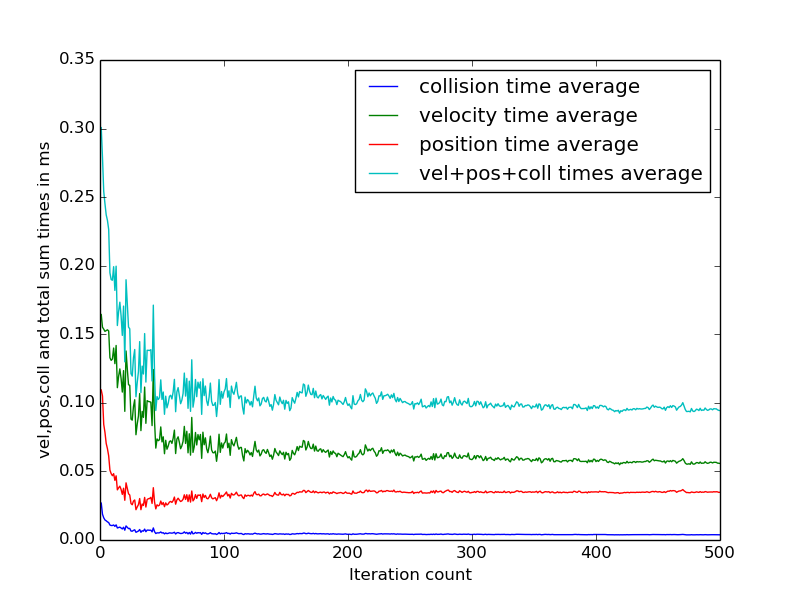
\includegraphics[scale=.60]{../images/plot02.png}
\caption{plot02}
\end{figure}

\par{Box2D uses constraint solver for solving constraints. The constraint solver solves all the constraints in the simulation, one at a time. Although single constraint can be solved perfectly, when we solve one constraint, we slightly disrupt other constraints. Therefore to get a good solution, we need to iterate over all constraints a number of times (in the same time step).}

\par{The time step and the iteration count are nearly unrelated. An iteration is not a sub-step. One solver iteration is a single pass over all the constraints within a time step.
There are two phases in the constraint solver: a velocity phase and a position phase. Each phase has its own iteration count. Here we are used velocity iterations=8 and position iterations=3.}

\par{This creates a trade-off between speed and accuracy. Using fewer iterations increases performance but accuracy suffers. Likewise, using more iterations decreases performance but improves the quality of your simulation. Since velocity iterations are more than position iterations, this acts as one of the factors in due to which time taken for velocity solving is more than that for position solving.}

\subsection{Observations from Step time average (error bars) vs No. of Iterations graph}
\begin{figure}[h!]
\centering
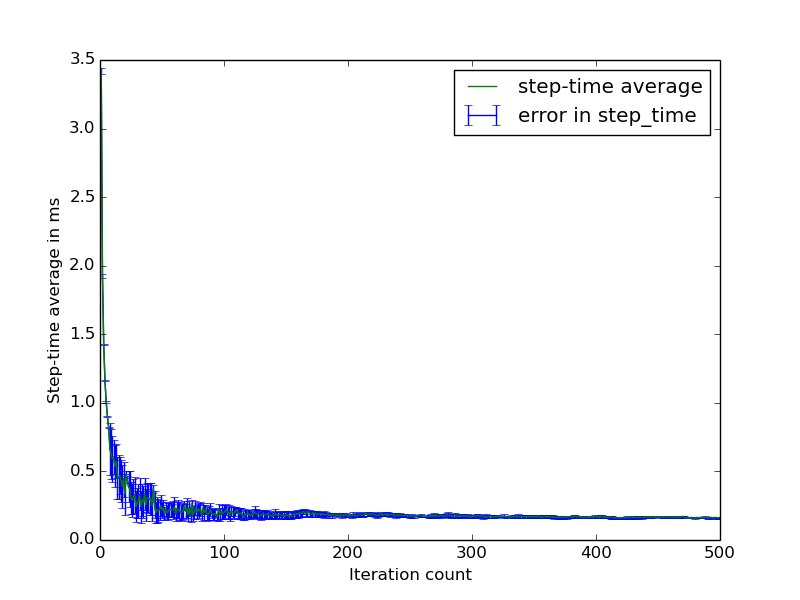
\includegraphics[scale=.60]{../images/plot03.png}
\caption{plot03}
\end{figure}
\indent 
\par{Note that the above plots represents average step time and y-error bars, the difference between the max and min values is large. Although the values are taken within 10 reruns, there are theses differences due to system processes. The errors decrease with increasing iteration count.}


\section{Profiling}

\subsection{perf}
\par{The profiler used for this task is perf\cite{perf}. The command perf report ./mybins/cs296\_09\_exe runs the executable and records samples required for profiling in a file perf.data. To generate human readable flat profile, the command perf record is used.}

\subsection{Release mode}
\par{For profiling in this mode, we use the cmake -DCMAKE\_BUILD\_TYPE=Release ../. command in Box2D installation. This is an out-of-source build.  An out-of-source build puts the files generated by the built in a completely separate directory, so that the source tree is unchanged. Also, the -O3 flag is used with gcc in code compilation.}

\subsubsection{Profiling Report}

\par{The executable ./mybins/cs296\_09\_exe was run with 5000 iterations of the for loop, and the output of perf report is shown in Figure 6.}

\par{The function which which makes up a large part of the running time is 0x2cf9b. As this is called from libm-2.15.so library, we can't optimize this. Functions operator+ and operator* are used for vector arithmetic. Function debug\_draw\_t takes up larger time than usual because we have edited debug\_draw in render.cpp to add custom colour particles (circles). Calls to constructor b2Vec2() are also high as a lot of coordinate positions (which are of type b2Vec2) are used in the code.} 

\par{Also, a number of functions have been inlined (because of -O3 optimization flag), so the function calls in the code have been replaced by the functions body. This means that the (percentage of) samples collected of the parent function will include the samples that should have been collected of the called function.}

\par{The column 'Overhead' indicates the percentage of the overall samples collected in the corresponding function. The second column reports the process from which the samples were collected. If a program is dynamically linked, then this shows the name of a shared library. When the samples come from the kernel, then the pseudo ELF image name [kernel.kallsyms] is used.}

\begin{figure}[h!]
\centering
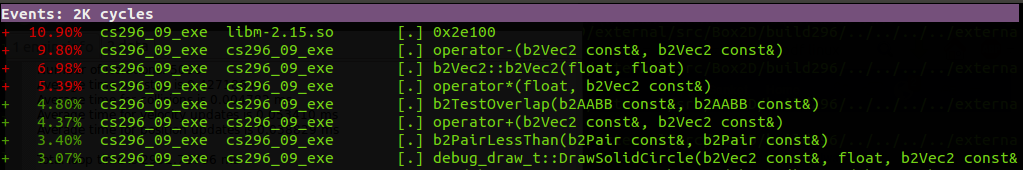
\includegraphics[scale=.43]{../images/release.png}
\caption{perf report in Release mode.}
\end{figure}

\subsubsection{Call graph}

\begin{figure}[h!]
\centering
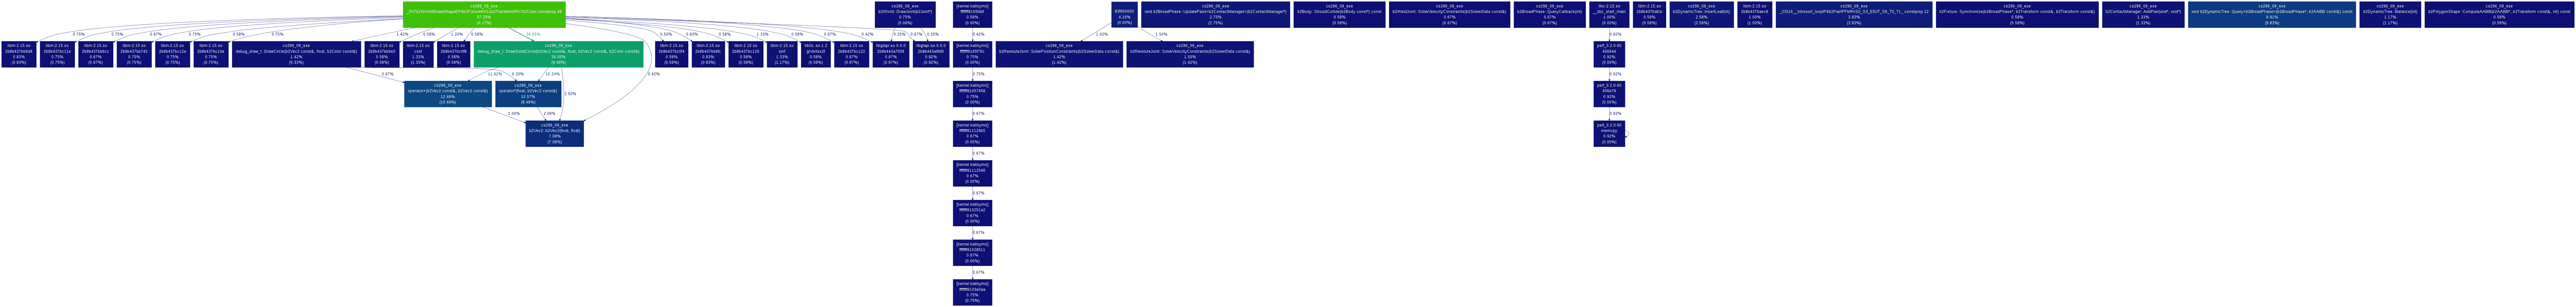
\includegraphics[scale=.06]{../images/releasecallgraph.png}
\caption{Call graph in release mode.}
\end{figure}

\subsection{Debugging mode}

\par{cmake -DCMAKE\_BUILD\_TYPE=Debug has been used in Box2D installation. This uses various debugging flags of the compiler. Also, compiler optimization options have been excluded. This means the debugging of the program will be easier, but at the expense of speed.}

\subsubsection{Profiling report}

\par{The executable ./mybins/cs296\_09\_exe was run with 5000 iterations of the for loop, and the output of +perf report is shown in Figure 6.}

\begin{figure}[h]
\centering
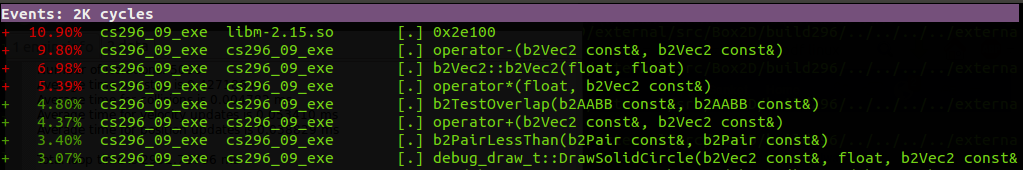
\includegraphics[scale=.43]{../images/debug.png}
\caption{perf report in Debug mode.}
\end{figure}

\par{This report is clearer than that produced in release mode. The highest overhead is from symbol 0x2e100, which is from the libm-2.15.so shared object. Other function calls whose overhead is high are: operator*, operator-, b2Vec2() etc. We must focus on optimizing (or reducing their number of calls of) the latter functions (which are part of Box2D), rather than trying to optimize the function 0x2e100, which is from a dynamic library.}

\subsubsection{Call graph}

\par{The call graph generated is shown in Figure 8. It can be easily seen that this has higher number of function calls (because compiler optimization options have not been used). Also, this graph is easier to understand (and to debug) than that produced in Release mode. Familiar functions like main(), b2ContactSolver(), b2World::Step() etc. can be identified easily.}

\begin{figure}[h!]
\centering
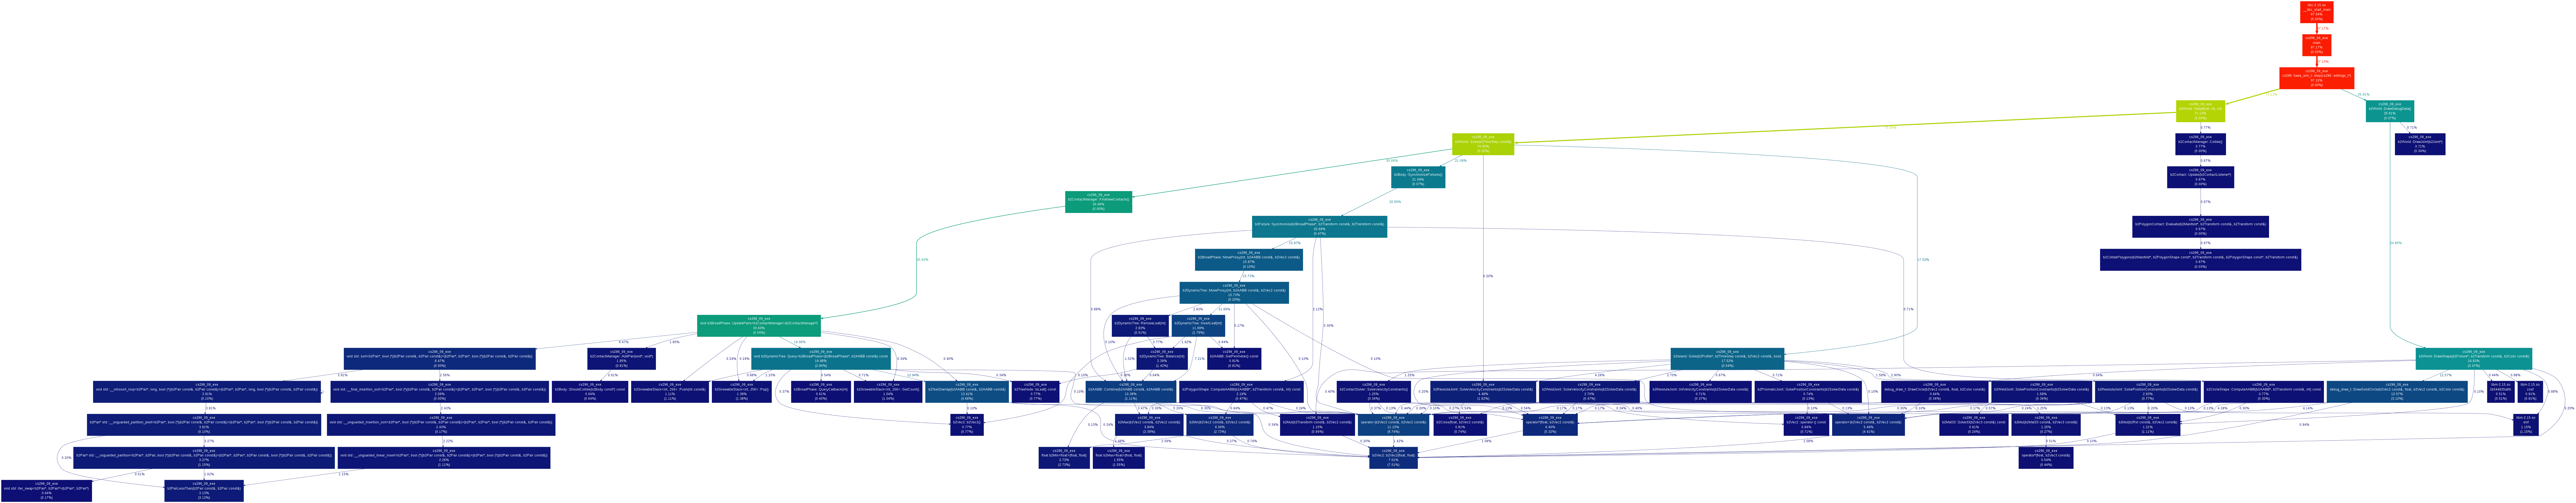
\includegraphics[scale=.044]{../images/debugcallgraph.png}
\caption{Call graph in Debug mode.}
\end{figure}

\bibliographystyle{plain}
\bibliography{cs296_report_project}

\end{document}